%%%%%%%%%%%%%%%%%%%%%%%%%%%%%% STANDARDS 5.0.1 section %%%%%%%%%%%%%%%%%%%%%%%%%%%%%%%%%
\section{Overview of the STANDARDS Database System}

The Spent Nuclear Fuel and Waste Disposition: Tracking, Analysis, and Reporting Database System (STANDARDS) is a comprehensive data
 management and analysis platform developed for the U.S. Department of Energy to support national fuel cycle studies, waste 
 management planning, and repository performance assessments. STANDARDS functions as a centralized, relational database that 
 integrates historical and projected inventories of spent nuclear fuel (SNF) and high-level radioactive waste (HLW) across 
 commercial and government sectors in the United States. The system is designed to provide consistent, traceable, and 
 physics-informed data products that can be used for systems analysis, policy evaluation, and fuel cycle modeling.

At its core, STANDARDS is implemented as a relational MySQL database coupled with a graphical user interface (GUI) that 
allows users to query, aggregate, and export inventory data. The database architecture organizes information into structured 
tables representing reactors, fuel assemblies, isotopic compositions, decay characteristics, storage configurations, and 
institutional ownership. While the GUI offers a user-friendly interface for exploratory analysis, the authoritative access 
method to the data is through direct SQL queries to the underlying database.

The primary unit of information in STANDARDS is the fuel assembly. Each spent fuel assembly is treated as a discrete entity 
associated with a specific reactor, assembly design, discharge date, burnup, enrichment, and heavy metal mass. Assemblies are 
indexed by reactor type (e.g., pressurized water reactor (PWR), boiling water reactor (BWR), gas-cooled reactors, experimental 
reactors), site location, and operational status. This assembly-level resolution enables detailed tracking of national 
inventories and allows inventories to be aggregated across multiple dimensions, such as by discharge year, reactor class, 
storage mode, or geographic region.

STANDARDS does not rely on direct isotopic measurements for every assembly. Instead, isotopic compositions are generated 
using physics-based depletion and decay models, primarily derived from ORIGEN-based libraries and burnup templates. For 
each assembly, isotopic vectors are calculated as functions of reactor type, burnup, initial enrichment, and cooling time. 
This approach ensures internal consistency and allows isotopic inventories to be projected forward in time. As a result, 
STANDARDS can provide isotopic compositions both at the time of discharge and after arbitrary decay periods, making it 
suitable for long-term storage and disposal analyses.

The isotopic data stored in STANDARDS includes detailed inventories of major actinides (U and Pu), minor actinides (Np, Am, Cm), 
and fission products. These data are essential for evaluating radiotoxicity, decay heat, neutron source terms, and transmutation 
potential. In addition to commercial light-water reactor fuel, the database also includes specialized inventories such as 
DOE-managed spent fuel, naval reactor fuel, research reactor fuel, and reprocessing waste streams. These inventories are 
stored in separate but compatible data structures, allowing them to be analyzed within the same framework as commercial SNF.

Beyond spent fuel, STANDARDS includes data for high-level waste generated from reprocessing activities at DOE sites and the 
former commercial reprocessing facility at West Valley, New York. These waste forms include vitrified waste canisters, 
calcined waste, cesium/strontium capsules, and metallic or ceramic waste forms from electrochemical processing. For these 
\materials, STANDARDS stores mass, radionuclide inventories, and decay heat characteristics, enabling assessments of repository 
thermal loading and waste packaging requirements.

The STANDARDS GUI provides a set of predefined query tools that allow users to generate common inventory reports, such as 
total SNF mass by year, inventory by reactor type, storage configuration (wet versus dry), or isotopic composition by burnup class. 
These tools are intended primarily for human users performing exploratory or policy-driven analyses. However, all GUI operations 
are internally implemented as SQL queries, and advanced users may access the database directly for customized analyses.

From a data access perspective, STANDARDS is fundamentally a database system rather than a static data product. The manual 
documents the database schema, field definitions, modeling assumptions, and usage methods, but does not contain the inventory data 
itself. To extract data, users must either use the Windows GUI or issue SQL queries against the database instance. This design 
supports reproducible, auditable workflows and enables integration with external modeling tools.

In the context of fuel cycle simulation, STANDARDS serves as a national inventory generator. It provides physically consistent, 
assembly-level isotopic vectors that can be aggregated into material streams for system-level models such as Cyclus. By querying 
STANDARDS for assemblies grouped by reactor type, discharge year, burnup, and cooling time, realistic material recipes 
representing U.S. spent fuel inventories can be constructed. These recipes can then be exported to CSV or similar formats and 
used directly as input materials in agent-based fuel cycle simulations.

Overall, STANDARDS functions as the authoritative digital representation of U.S. spent nuclear fuel and high-level waste 
inventories. Its primary contribution is the integration of historical operational data with physics-based isotopic modeling in 
a single, queryable database. The system is designed to support national-scale analyses of storage, disposal, reprocessing, and 
transmutation strategies, and it provides a critical data foundation for advanced fuel cycle modeling and decision support studies.

%%%%%%%%%%%%%%%%%%%%%%%%%%%%%%%%%%%%%%%%%%%%%%%%%%%%%%%%%%%%%%%%%%%%%%%%%%%%%%%%%%%%%%%%%%%%%%%%%%%%%%%%%%%%%%%%%%%%%%%%%%%%%%%%%%%%%%%%%%%%%%%%%%%%%%%%%%%%%%%%%%%%%
%%%%%%%%%%%Additional Capability Being Developed from UNF-ST&DARDS Unified Database: System Analysis and Fuel Cycle Option Analysis%%%%%%%%%%%%%%%%%%%%%%%%%%%%%%%%%
\section{Summary of UNF-ST\&DARDS Capabilities for System and Fuel Cycle Analysis}

The Used Nuclear Fuel Storage, Transportation \& Disposal Analysis Resource and Data System (UNF-ST\&DARDS) is a comprehensive 
analysis framework developed for the U.S. Department of Energy to support long-term planning and decision-making for spent nuclear 
fuel (SNF) management. A core component of this system is the Unified Database (UDB), which represents the most extensive and 
detailed database of commercial SNF in the United States. The UDB integrates data from multiple sources, including the EIA GC-859 
survey, utility-provided information, vendor data, and calculated results from nuclear analysis tools such as SCALE and COBRA-SFS.

The UDB contains a wide range of datasets, including assembly-level information such as burnup, enrichment, discharge dates, 
and reactor type, as well as cask and canister attributes, transportation infrastructure data, site characteristics, and 
economic parameters. In addition, the database includes calculated neutronic, thermal, shielding, and criticality properties. 
These data allow detailed characterization of SNF assemblies and storage systems, including radionuclide inventories, decay heat, 
dose rates, and thermal performance, enabling high-fidelity technical assessments of storage, transportation, and disposal options.

One major application of the UDB is system-level analysis through the Next-Generation System Analysis Model (NGSAM), 
an agent-based, discrete-event simulation tool designed to model the full waste management system. NGSAM uses UDB data to 
simulate the movement of SNF from reactors to interim storage facilities and ultimately to geological repositories. It incorporates 
realistic operational constraints and transportation logistics, allowing analysts to evaluate scenarios involving storage capacity, 
shipment schedules, repackaging operations, and system bottlenecks over long time horizons.

A second major application of the UDB is fuel cycle analysis. Assembly-specific radionuclide inventories are generated within 
UNF-ST\&DARDS using SCALE depletion and decay calculations. These calculations provide isotopic compositions, decay heat, 
and activity for each individual assembly as a function of time. This capability enables detailed modeling of material flows 
for advanced fuel cycle scenarios, such as recycling plutonium and minor actinides into fast reactors or accelerator-driven systems, 
using realistic isotopic vectors derived directly from the national SNF inventory.

The paper highlights a key advancement in directly coupling UDB isotopic data to fuel cycle simulators such as ORION. 
This approach improves accuracy compared to traditional static ``recipe'' methods, which rely on average discharge compositions 
and do not capture variations in enrichment, burnup, and discharge timing. The UDB-based approach preserves assembly-level 
resolution while maintaining reasonable computational cost, leading to more realistic predictions of plutonium, uranium, 
minor actinide, and fission product inventories.

Overall, the UNF-ST\&DARDS Unified Database serves as a national reference dataset that enables integrated system analysis 
and advanced fuel cycle modeling. By linking detailed SNF data with simulation tools such as NGSAM and ORION, the framework 
supports more credible evaluations of storage, transportation, disposal strategies, and future fuel cycle transitions, 
providing a robust technical foundation for long-term nuclear waste management decision-making.

%%%%%%%%%%%%%%%%%%%%%%%%%%%%%%%%%%%%%%%%%%%%%%%%%%%%%%%%%%%%%%%%%%%%%%%%%%%%%%%%%%%%%%%%%%%%%%%%%%%%%%%%%%%%%%%%%%%%%%%%%%%%%%%%%%%%%%%%%%%%%%%%%%%%%%%%%%%%%%%%%%%%%
%%%%%%%%%%%%%%%%%%%%%%%%%%%%%%%%%Flexibility of ADS for minor actinides transmutation in different two-stage PWR-ADS fuel cycle scenarios%%%%%%%%%%%%%%%%%%%%%%%%%%%%%%%%%
\subsection{Flexibility of ADS for Minor Actinide Transmutation}

Accelerator Driven Systems (ADS) have been widely proposed as a promising option for the transmutation of minor actinides (MAs) 
recovered from spent light water reactor (LWR) fuel, due to their inherent subcritical operation and favorable neutron economy. 
In this work, a two-stage PWR--ADS fuel cycle is analyzed, where MAs are first separated from spent pressurized water reactor (PWR) 
fuel and subsequently transmuted in an ADS system. The spent ADS fuel is then reprocessed using a pyro-chemical process, and the 
recovered actinides are recycled back into the ADS core together with additional MAs recovered from PWR spent fuel.

The study evaluates the flexibility of the ADS system under three key aspects: (1) cooling time of spent ADS fuel prior to 
reprocessing, (2) reprocessing loss of actinides in the pyro-chemical process, and (3) variation in MA composition originating 
from different types of spent PWR fuels. A three-dimensional neutronics and depletion model is employed using coupled Monte Carlo 
transport and core analysis tools, considering detailed actinide and fission product inventories.

Results indicate that increasing the cooling time of spent ADS fuel leads to a higher required heavy metal inventory in the 
ADS core, as short-lived fissile isotopes such as \textsuperscript{238}Pu and \textsuperscript{241}Pu decay into less reactive 
nuclides. However, the overall transmutation performance, measured in terms of long-term decay heat and radiotoxicity reduction, 
is only weakly affected by the cooling time, demonstrating that ADS performance is robust with respect to realistic cooling 
constraints.

The impact of reprocessing loss is found to be more significant in determining long-term waste reduction performance. While 
reprocessing losses have minimal effect on reactor neutronic parameters, they strongly influence the achievable reduction in 
decay heat and radiotoxicity of minor actinides. The study shows that meaningful long-term waste reduction requires reprocessing 
losses to be maintained below approximately 0.2\%, highlighting the importance of efficient pyro-chemical separation technologies.

Finally, the ADS system is shown to be flexible with respect to different MA feed compositions derived from various spent 
PWR fuels, including UOX and MOX fuel cycles. Although some variations in core inventory and burnup performance are observed, 
the overall transmutation effectiveness remains comparable across different feed scenarios. The results confirm that ADS can 
effectively transmute a wide range of MA vectors, making it a robust and adaptable technology for advanced fuel cycle strategies 
focused on long-term waste minimization.

%%%%%%%%%%%%%%%%%%%%%%%%%%%%%%%%%%%%%%%%%%%%%%%%%%%%%%%%%%%%%%%%%%%%%%%%%%%%%%%%%%%%%%%%%%%%%%%%%%%%%%%%%%%%%%%%%%%%%%%%%%%%%%%%%%%%%%%%%%%%%%%%%%%%%%%%%%%%%%%%%%%%%
%%%%%%%%%%%%%%%%%%%%%%%%%%%%%%%%%Accelerator-driven systems%%%%%%%%%%%%%%%%%%%%%%%%%%%%%%%%%%%%%%%%%%%%%%%%%%%%%%%%%%%%%%%%
\section{Accelerator-Driven Systems (ADS) for Minor Actinide Transmutation}

\subsection{Introduction and Motivation}

Accelerator-Driven Systems (ADS) are subcritical nuclear systems coupled to an external neutron source, typically provided by a 
high-power particle accelerator. ADS concepts have been extensively studied as a potential technology for the transmutation of 
long-lived radionuclides, particularly minor actinides (MAs), in order to reduce the long-term radiotoxicity and heat load of 
spent nuclear fuel (SNF). Unlike critical reactors, ADS operate with an effective multiplication factor $k_{\text{eff}} < 1$, 
which enhances inherent safety characteristics and allows for operation with fuel compositions containing high fractions of 
actinides that would be difficult or unsafe to sustain in critical systems.

The primary motivation for ADS development lies in fuel cycle closure strategies, where plutonium and minor actinides are 
recycled and transmuted to shorter-lived or stable isotopes. This approach aims to mitigate the challenges associated with 
geological disposal by reducing both the radiological hazard and the required isolation time of nuclear waste.

\subsection{Physical Principle of Subcritical Operation}

In an ADS, fission reactions are sustained by an external neutron source rather than by a self-sustaining chain reaction. 
The system remains subcritical at all times, satisfying:

\begin{equation}
k_{\text{eff}} < 1
\end{equation}

The neutron population $N$ in the system is governed by the balance between the externally supplied source neutrons and the 
internally generated fission neutrons. The subcritical multiplication factor $M$ is defined as:

\begin{equation}
M = \frac{1}{1 - k_{\text{eff}}}
\end{equation}

This expression shows that as $k_{\text{eff}}$ approaches unity, the neutron amplification increases significantly, 
enhancing system power for a fixed external source strength. However, the system remains inherently safe since any 
interruption in the accelerator beam immediately terminates the neutron supply.

The total thermal power of the ADS can be approximated by:

\begin{equation}
P = S_n \cdot M \cdot E_f
\end{equation}

where $S_n$ is the external neutron source intensity (neutrons per second), $M$ is the subcritical multiplication factor, 
and $E_f$ is the average energy released per fission event.

\subsection{Spallation Neutron Source}

The external neutron source in ADS is typically generated through spallation reactions, where high-energy protons 
(on the order of 0.8--1.5 GeV) strike a heavy metal target such as lead, tungsten, or lead-bismuth eutectic (LBE). 
The spallation process can be represented schematically as:

\begin{equation}
p + A \rightarrow A^* + x n + y p + z \pi
\end{equation}

where $p$ is the incident proton, $A$ is the target nucleus, and multiple neutrons $n$ are emitted.

The average neutron yield per proton is approximately:

\begin{equation}
Y_n \approx 20 - 30 \quad \text{neutrons per proton at } 1 \text{ GeV}
\end{equation}

The spallation target must withstand extremely high thermal and radiation loads, making target material selection and 
thermal-hydraulic design critical engineering challenges.

\subsection{Accelerator Requirements}

ADS concepts require a high-power, continuous-wave proton accelerator capable of delivering beam currents on the order of 
several milliamperes at GeV-scale energies. Typical design parameters include:

\begin{itemize}
\item Proton energy: 0.8--1.5 GeV
\item Beam current: 5--20 mA
\item Beam power: 5--30 MW
\end{itemize}

High reliability is a fundamental requirement, as frequent beam trips can induce large thermal stresses in reactor components. 
Acceptable beam interruption frequencies are generally below a few events per year, imposing stringent operational constraints on 
accelerator technology.

\subsection{Neutronics and Transmutation Performance}

The primary objective of ADS systems in waste management applications is the transmutation of minor actinides such as:

\begin{itemize}
\item Neptunium-237
\item Americium-241, Americium-243
\item Curium-244, Curium-245, Curium-246
\end{itemize}

The transmutation rate $R_i$ for a given isotope $i$ can be expressed as:

\begin{equation}
R_i = \phi \cdot \sigma_i \cdot N_i
\end{equation}

where $\phi$ is the neutron flux, $\sigma_i$ is the effective reaction cross section, and $N_i$ is the number density of 
isotope $i$.

High neutron fluxes ($\sim 10^{15}$--$10^{16}$ n/cm$^2$/s) are achievable in ADS cores, enabling efficient destruction of 
long-lived actinides. The resulting isotopic evolution typically leads to:

\begin{itemize}
\item Reduction in Am and Cm inventories
\item Conversion of Np-237 into shorter-lived plutonium isotopes
\item Accumulation of fission products
\end{itemize}

\subsection{Molten Salt ADS Concepts}

One prominent class of ADS designs involves molten salt fuel, where actinide fluorides are dissolved directly in a 
carrier salt such as FLiBe (LiF-BeF$_2$) or FLiNaK (LiF-NaF-KF). In these systems, fuel circulates continuously through the core, 
enabling online processing and removal of fission products.

The molten salt approach offers several advantages:

\begin{itemize}
\item Excellent heat transfer properties
\item Homogeneous fuel composition
\item Capability for continuous reprocessing
\item Enhanced flexibility in fuel loading
\end{itemize}

The effective multiplication factor in molten salt ADS is typically maintained in the range:

\begin{equation}
0.95 \leq k_{\text{eff}} \leq 0.98
\end{equation}

which balances high neutron economy with strong subcritical safety margins.

\subsection{Safety and Control Characteristics}

ADS systems exhibit fundamentally different safety behavior compared to critical reactors. Since the system is externally driven, 
the power level is directly proportional to the accelerator beam current:

\begin{equation}
P(t) \propto I_{\text{beam}}(t)
\end{equation}

This allows for rapid and precise power control through beam modulation. In the event of accelerator shutdown, fission reactions 
cease almost instantaneously, leaving only decay heat.

Reactivity feedback mechanisms still exist, including Doppler broadening and thermal expansion, but the absence of prompt 
criticality eliminates many of the accident scenarios associated with conventional reactors.

\subsection{Fuel Cycle Implications}

From a fuel cycle perspective, ADS systems enable a partitioning and transmutation strategy in which:

\begin{enumerate}
\item Spent nuclear fuel is reprocessed.
\item Minor actinides are separated.
\item MAs are fed into ADS for destruction.
\item Remaining materials are directed to storage or reuse.
\end{enumerate}

The effectiveness of ADS transmutation is often measured using metrics such as:

\begin{itemize}
\item Actinide mass reduction fraction
\item Radiotoxicity reduction factor
\item Decay heat reduction
\item Repository loading benefit
\end{itemize}

Studies consistently show that ADS-based fuel cycles can reduce long-term radiotoxicity by one to two orders of magnitude and 
shorten required isolation times from hundreds of thousands of years to a few thousand years.

\subsection{Relevance to This Work}

In the context of this research, ADS models provide the physical basis for implementing transmutation facilities within Cyclus. 
The isotopic destruction rates, neutron economy, and material flow characteristics described in ADS literature directly inform the 
design of XDS facility archetypes. By coupling realistic ADS performance models with national spent fuel inventories, system-level 
impacts of advanced transmutation strategies can be quantitatively assessed.

%%%%%%%%%%%%%%%%%%%%%%%%%%%%%%%%%%%%%%%%%%%%%%%%%%%%%%%%%%%%%%%%%%%%%%%%%%%%%%%%%%%%%%%%%%%%%%%%%%%%%%%%%%%%%%%%%%%%%%%%%%%%%%%%%%%%%%%%%%%%%%%%%%%%%%%%%%%%%%%%%%%%%
%%%%%%%%%%%%%%%%%%%%%%%%%%%%%%%%%Nuclear data sensitivity, uncertainty and target accuracy assessment for future nuclear systems%%%%%%%%%%%%%%%%%%%%%%%%%%%%%%%%%%%%%%%%%%%%%%%%%%%%%%%%%%%%%%%%

\subsection{Aliberti et al. (2006): Nuclear Data Sensitivity and Uncertainty for Future Systems}
\label{subsec:aliberti2006}

Aliberti et al. (2006) present a comprehensive sensitivity and uncertainty (S\&U) analysis framework aimed at quantifying the 
impact of nuclear data uncertainties on the performance and safety-related parameters of advanced nuclear systems, particularly 
those envisioned within the Generation IV (Gen IV) and Advanced Fuel Cycle Initiative (AFCI) programs. The study addresses a 
critical issue in reactor physics and fuel cycle analysis: while modern nuclear data libraries provide extensive evaluated 
cross-section datasets, the associated uncertainties and correlations remain a major source of epistemic uncertainty in the 
predictive capability of advanced reactor simulations.

\textbf{Objective and Scope.}  
The primary objective of the study is to assess how uncertainties in neutron-induced reaction cross sections propagate into 
uncertainties in key integral parameters of future nuclear systems. These parameters include the effective multiplication 
factor ($k_{\text{eff}}$), temperature and coolant void reactivity coefficients, burnup reactivity swing, isotopic inventories at 
end-of-cycle, decay heat, neutron source terms, and long-term radiotoxicity. The analysis is intended to support feasibility and 
design optimization studies for innovative reactors and closed fuel cycles, with a particular focus on systems involving fast 
spectra and minor actinide (MA) recycling.

Six representative reactor systems are considered: a Gas-cooled Fast Reactor (GFR), a Lead-cooled Fast Reactor (LFR), a 
Sodium-cooled Fast Reactor in burner configuration (SFR), a large Sodium-cooled Fast Reactor with breeding capability (EFR), 
a Very High Temperature Reactor (VHTR) with TRISO fuel, and an extended burnup Pressurized Water Reactor (PWR). These systems 
span a wide range of neutron spectra, fuel types, and fuel cycle strategies, allowing the authors to draw general conclusions 
applicable to both fast and thermal systems.

\textbf{Methodology: Sensitivity and Uncertainty Framework.}  
The study employs generalized perturbation theory (GPT) to compute sensitivity coefficients, which quantify the relative 
change in an integral parameter $R$ due to a relative change in a nuclear data parameter $\sigma_{i,x,g}$ 
(cross section of isotope $i$, reaction type $x$, and energy group $g$). The uncertainty in an integral parameter is then 
obtained via quadratic propagation using a variance-covariance matrix $D$:
\[
(\Delta R)^2 = \mathbf{S}_R^T \, \mathbf{D} \, \mathbf{S}_R,
\]
where $\mathbf{S}_R$ is the sensitivity vector.

Sensitivity calculations are performed using the ERANOS code system, which solves the Boltzmann transport equation and 
the associated adjoint equations in multi-group form. Time-dependent sensitivities for nuclide transmutation and decay-related 
quantities are computed using the NUTS module, while decay heat calculations rely on ORIGEN. This integrated deterministic 
framework allows the authors to evaluate a wide spectrum of integral parameters within a consistent theoretical and computational 
setting.

A key methodological contribution of the paper is the construction and use of two alternative covariance datasets: 
(1) the so-called \emph{ANL covariance matrix}, which is a semi-empirical covariance set derived from the analysis of clean 
integral experiments (e.g., PHENIX irradiation experiments such as PROFIL and TRAPU), and (2) the \emph{NEA-K covariance matrix}, 
which is assembled from evaluated covariance data available at the OECD/NEA Data Bank. The ANL covariance matrix incorporates 
partial energy correlations by grouping energy ranges into five broad bands, thereby introducing physically motivated correlations 
across energy groups.

\textbf{Uncertainty Sources and Covariance Data.}  
The authors devote significant attention to the issue of nuclear data covariance, emphasizing that realistic 
uncertainty quantification requires not only diagonal uncertainties but also energy correlations. For major 
actinides (e.g., $^{235}$U, $^{238}$U, $^{239}$Pu), uncertainties are constrained using extensive criticality benchmarks 
and irradiation experiments. For minor actinides (e.g., Np, Am, Cm isotopes), the available integral information is more limited, 
especially in fast spectra, leading to larger epistemic uncertainty.

Fission product (FP) data uncertainties are treated in a simplified manner using a ``lumped fission product'' approach, with 
capture cross-section uncertainties of approximately 10\% for fast systems and 2\% for thermal systems. Structural and coolant 
materials (e.g., Fe, Pb, Na) are assigned uncertainties based on discrepancies among evaluated libraries and limited experimental 
evidence, highlighting the preliminary nature of these estimates.

The comparison between the ANL and NEA-K covariance matrices reveals substantial inconsistencies in evaluated covariance data. 
In particular, some evaluated datasets exhibit unrealistically small uncertainties for important reactions (e.g., $^{241}$Pu 
fission or $^{239}$Pu capture), which are not supported by integral experiment performance. This finding underscores the need for 
improved covariance evaluations and systematic validation against integral benchmarks.

\textbf{Key Results and Findings.}  
The uncertainty analysis shows that nuclear data uncertainties are significant only for a limited subset of integral parameters. 
The most affected quantities are:
\begin{itemize}
    \item The effective multiplication factor $k_{\text{eff}}$ for all systems.
    \item Burnup reactivity swing and associated isotopic inventories.
    \item Coolant void coefficients in fast reactors.
    \item Neutron source terms at fuel discharge in thermal systems.
\end{itemize}

For other parameters, such as peak power, decay heat at 100 years, and long-term radiotoxicity, uncertainties remain 
within anticipated target accuracies and are therefore less critical from a design perspective.

Across all systems, the dominant contributors to uncertainty in $k_{\text{eff}}$ are still $^{238}$U capture and $^{239}$Pu 
fission and capture reactions, even in reactors with substantial minor actinide loading. This result indicates that, despite the 
increased role of MAs in advanced fuel cycles, the overall system uncertainty remains largely driven by major actinide nuclear data.

Energy-dependent analyses further show that the most influential energy ranges are:
\begin{itemize}
    \item Fast energies (1 MeV to 1 keV) for $^{239}$Pu fission.
    \item Epithermal and resonance ranges for $^{238}$U capture.
    \item First resonance region for $^{240}$Pu capture.
\end{itemize}

Minor actinide reactions play a secondary role, with notable exceptions such as $^{241}$Am capture in the GFR and $^{242m}$Am 
fission in the SFR. However, even in these cases, MA uncertainties do not dominate the global uncertainty budget.

\textbf{Target Accuracy Assessment and Implications.}  
An important contribution of the paper is the formulation of a target accuracy assessment problem, in which required 
improvements in nuclear data are derived from target accuracies on integral design parameters. This is framed as an 
optimization problem that balances the ``cost'' of improving specific nuclear data against their impact on reducing 
system-level uncertainty.

The results indicate that priority should be given to improving:
\begin{itemize}
    \item $^{238}$U capture cross sections.
    \item $^{239}$Pu fission and capture data.
    \item Selected structural material cross sections in fast systems.
\end{itemize}

In contrast, further refinement of minor actinide data is of secondary importance from a system uncertainty perspective, 
although such improvements remain relevant for transmutation performance and waste management studies.

\textbf{Significance and Relevance.}  
This work represents one of the most systematic and comprehensive applications of sensitivity and uncertainty analysis to 
advanced nuclear systems. Its main significance lies in demonstrating that nuclear data uncertainties, while non-negligible, 
do not fundamentally compromise the feasibility of Generation IV reactor concepts. Instead, uncertainties are concentrated in a 
few well-identified reactions and energy ranges, enabling targeted experimental and evaluation efforts.

For advanced fuel cycle modeling and system-level simulators such as Cyclus, this study provides a strong theoretical 
justification for prioritizing uncertainty propagation and for focusing nuclear data improvement efforts on major actinide 
reactions. Moreover, the methodological framework established by Aliberti et al. remains highly relevant for modern uncertainty 
quantification workflows, including hybrid deterministic–stochastic approaches and Bayesian data assimilation techniques.

Overall, the paper establishes sensitivity and uncertainty analysis as an indispensable tool for credible assessment of 
future nuclear systems and offers clear guidance on where nuclear data improvements would yield the greatest benefit in terms of 
reducing predictive uncertainty.
%%%%%%%%%%%%%%%%%%%%%%%%%%%%%%%%%%%%%%%%%%%%%%%%%%%%%%%%%%%%%%%%%%%%%%%%%%%%%%%%%%%%%%%%%%%%%%%%%%%%%%%%%%%%%%%%%%%%%%%%%%%%%%%%%%%%%%%%%%%%%%%%%%%%%%%%%%%%%%%%%%%%%
%%%%%%%%%%%%%%%%%%%%%%%%%%%%%%%%%ADS design concept for disposing of the U.S. spent nuclear fuel inventory%%%%%%%%%%%%%%%%%%%%%%%%%%%%%%%%%%%%%%%%%%%%%%%%%%%%%%%%%%%%%%%%
\subsection{Gohar et al. (2021): ADS Design Concept for Disposing of the U.S. Spent Nuclear Fuel Inventory}
\label{subsec:gohar2021}

Gohar et al. (2021) propose a comprehensive conceptual design of an accelerator-driven subcritical (ADS) system aimed at 
disposing of the entire United States spent nuclear fuel (SNF) inventory through the utilization and transmutation of minor 
actinides (MAs) and selected long-lived fission products (LLFPs). The study represents one of the most detailed and system-level 
ADS design efforts in the open literature, integrating neutronics, burnup, and thermal--hydraulic analyses into a single consistent 
engineering framework. The work is motivated by the long-term challenge of managing approximately 80,000 metric tons of heavy metal 
(MTHM) of SNF in the U.S., which contains about 131 tons of MAs and roughly 669 tons of plutonium.

\textbf{Motivation and System-Level Objective.}  
The central objective of the study is to design an ADS system capable of:
\begin{itemize}
    \item Utilizing the MA inventory extracted from U.S. SNF as a primary fuel source.
    \item Producing useful thermal power while remaining deeply subcritical.
    \item Transmuting a fraction of long-lived fission products (notably $^{99}$Tc and $^{129}$I).
    \item Achieving full disposal of the U.S. SNF inventory using a small number of identical ADS units.
\end{itemize}

The authors emphasize that traditional repository-based disposal strategies face significant political, technical, and 
societal challenges, and that advanced nuclear systems capable of reducing the long-term radiotoxicity and heat load of 
SNF may offer a complementary or alternative solution. Unlike many prior ADS studies that rely on solid fuel forms, this 
work explores a mobile liquid fuel concept, which avoids the need for new solid MA-bearing fuel fabrication technologies and 
simplifies fuel handling and reprocessing.

\textbf{Spent Fuel Processing and Fuel Composition.}  
The ADS fuel is assumed to be derived from a single reprocessing step applied to LWR SNF with 25 years of cooling time, in 
which 99.995\% of uranium and short-lived fission products are removed. The resulting heavy metal composition used as input 
fuel consists of approximately:
\begin{itemize}
    \item 84.47\% plutonium,
    \item 5.02\% $^{237}$Np,
    \item 9.91\% americium,
    \item 0.12\% curium,
    \item 0.48\% residual uranium.
\end{itemize}

The fuel is divided into two conceptual streams: a plutonium-rich stream and a minor actinide stream. Since the primary 
objective is MA transmutation, plutonium is introduced only to the extent necessary to sustain sufficient neutron multiplication 
in the subcritical assembly. No isotopic enrichment or separation is assumed, and the analysis relies entirely on realistic 
compositions derived from standard SNF processing.

\textbf{Spallation Neutron Source and Accelerator Parameters.}  
The system is driven by a high-power spallation neutron source generated by a 1-GeV proton beam striking a liquid lead or 
lead--bismuth eutectic (LBE) target. Monte Carlo simulations show that approximately 15--16 neutrons are produced per incident 
proton, with the neutron yield saturating above 1 GeV. A beam power of 25 MW is selected, which corresponds to a proton current 
of 25 mA.

The spallation target is designed as a cylindrical liquid metal assembly with a hemispherical beam window and internal 
flow channels. Detailed thermal--hydraulic analyses using STAR-CCM+ demonstrate that the target can safely remove the 
deposited heat while maintaining structural temperatures below material limits, with peak window temperatures remaining 
well below 873 K. The use of liquid lead rather than LBE is ultimately favored to avoid the production of $^{210}$Po and to 
reduce corrosion and material compatibility issues.

\textbf{Homogeneous Fission Blanket Concept.}  
The first examined configuration is a homogeneous subcritical fission blanket, in which actinide fuel is dissolved or suspended 
in a liquid metal carrier (LBE or lead). The fission blanket surrounds the spallation target and acts as both fuel and primary 
coolant. Neutronics calculations indicate that to achieve a target effective multiplication factor of $k_{\text{eff}} = 0.98$, 
the required plutonium fraction ranges from approximately 40 at\% for low actinide loading (2\%) to around 13 at\% for higher 
actinide loading (10\%).

Parametric analyses show that a $k_{\text{eff}}$ value of 0.98 allows a thermal power of approximately 3 GW to be generated 
from a 25 MW proton beam, implying an energy amplification factor of about 120. Burnup simulations using the MCB5 code reveal 
that such systems can transmute between 30 and 37 tons of minor actinides over 35 full-power years, depending on fuel loading.

However, the homogeneous configuration suffers from severe engineering drawbacks. In particular, the required fuel inventory 
exceeds 40 tons of heavy metal, with more than 70 m$^3$ of liquid fuel circulating outside the core. This large inventory poses 
safety concerns, complicates chemical control, and makes early deployment impractical given realistic SNF processing rates.

\textbf{Inverted Bundle Fission Blanket.}  
To reduce fuel inventory and improve engineering feasibility, the authors propose an inverted bundle concept in which the 
slurry fuel fills the vessel, while the primary coolant flows inside thousands of small vertical tubes embedded in the fuel region.
 Heat is removed through these tubes to external heat exchangers, and only a small fraction of the fuel is circulated externally 
 for chemical processing and feeding.

This configuration drastically reduces the required MA inventory to about 12--13 tons per system and allows operation to 
begin within a few years of SNF processing. However, it introduces major mechanical challenges: more than 13,000 thin coolant 
tubes are required, creating significant fabrication, spacing, and thermal expansion difficulties. The large number of structural 
components also leads to increased neutron absorption and reduced system power.

\textbf{Final Bundle Fission Blanket Design.}  
The final and preferred configuration is the bundle concept, in which the roles of fuel and coolant are reversed: slurry fuel 
flows inside vertical tubes, while liquid lead coolant fills the surrounding tank. Tube diameters are varied radially, with 
smaller tubes near the spallation target where power density is highest, and larger tubes further away.

This design offers several key advantages:
\begin{itemize}
    \item Substantial reduction in the number of tubes (about 40\% fewer than the inverted bundle).
    \item Improved thermal--hydraulic performance with peak fuel tube surface temperatures below 873 K.
    \item More uniform power and temperature distributions.
    \item Reduced fuel inventory while maintaining high transmutation rates.
\end{itemize}

Full three-dimensional coupled MCNPX--STAR-CCM+ simulations show that the system operates safely with a coolant outlet 
temperature of approximately 730 K and a pressure drop of about 113 kPa. Flow zoning techniques further improve thermal 
efficiency by increasing outlet temperature by up to 36\% and reducing pumping power.

\textbf{Burnup and Transmutation Performance.}  
Burnup simulations are performed using both MCB5 and Serpent, with detailed spallation neutron source files generated by MCNPX. 
The fuel is managed through batch feeding every 90 days to maintain $k_{\text{eff}} \approx 0.98$. When reactivity increases 
due to the buildup of $^{242m}$Am, LLFP absorbers such as $^{99}$Tc and $^{129}$I are introduced. When reactivity decreases 
due to fissile depletion, fresh actinides are added.

The results show that each ADS unit can transmute approximately 30--37 tons of minor actinides over 35 years of operation. 
Consequently, the entire U.S. MA inventory of about 131 tons can be disposed of using approximately five identical ADS systems. 
The annual MA transmutation rate stabilizes at roughly 1 ton per year per system after an initial transient period.

\textbf{Significance and Implications.}  
This study represents one of the most realistic and integrated ADS design analyses available in the literature. Its main 
contribution is demonstrating, at a system level, that:
\begin{itemize}
    \item ADS-based disposal of national-scale SNF inventories is technically feasible.
    \item Minor actinides can be efficiently utilized as fuel in subcritical systems.
    \item Mobile liquid fuel concepts offer major advantages in flexibility, safety, and fuel cycle integration.
    \item A small fleet (on the order of five units) could, in principle, eliminate the long-term MA burden of the U.S. 
    nuclear fuel cycle.
\end{itemize}

For advanced fuel cycle modeling frameworks such as Cyclus, this work provides a rare example of a fully specified transmutation 
facility, including realistic neutronics, burnup behavior, and engineering constraints. It thus serves as a foundational reference 
for system-level studies of ADS deployment, waste minimization strategies, and closed fuel cycle architectures.


%%%%%%%%%%%%%%%%%%%%%%%%%%%%%%%%%%%%%%%%%%%%%%%%%%%%%%%%%%%%%%%%%%%%%%%%%%%%%%%%%%%%%%%%%%%%%%%%%%%%%%%%%%%%%%%%%%%%%%%%%%%%%%%%%%%%%%%%%%%%%%%%%%%%%%%%%%%%%%%%%%%%%
%%%%%%%%%%%%%%%%%%%%%%%%%%%%%%%%FundamentalconceptsintheCyclusnuclearfuelcyclesimulationframework%%%%%%%%%%%%%%%%%%%%%%%%%%%%%%%%%%%%%%%%%%%%%%%%%%%%%%%%%%%%%%%%
\subsection{Huff et al. (2016): Fundamental Concepts in the Cyclus Fuel Cycle Simulation Framework}
\label{subsec:huff2016}

Huff et al. (2016) present the fundamental design principles, architecture, and modeling philosophy of the Cyclus nuclear fuel 
cycle simulation framework. This work constitutes the primary methodological reference for Cyclus and establishes the conceptual 
foundations of a new generation of fuel cycle simulators based on agent-based modeling (ABM), discrete resource tracking, and 
modular software architecture. Unlike earlier fuel cycle simulators, which are often monolithic, closed-source, and limited in 
extensibility, Cyclus is explicitly designed as an open, flexible, and community-driven platform for modeling nuclear energy systems 
across a wide range of fidelities and scales.

\textbf{Motivation and Historical Context.}  
The authors situate Cyclus within the historical development of nuclear fuel cycle simulators, including national laboratory tools 
such as VISION, DYMOND, NFCSim, COSI, ORION, and DANESS. While these tools have supported important system-level analyses, they 
exhibit three fundamental limitations: (1) restricted accessibility and distribution, (2) limited support for user-driven extension 
and customization, and (3) difficulty in directly comparing alternative modeling methodologies due to tightly coupled, non-modular 
designs :contentReference[oaicite:1]{index=1}.

The U.S. DOE Fuel Cycle Technologies Systems Analysis Campaign formally identified these issues as critical barriers to scientific 
transparency, collaboration, and methodological innovation. In response, Cyclus was conceived to break from the traditional system 
dynamics paradigm and adopt a modern software engineering approach rooted in object-oriented design, modularity, and open 
development practices.

\textbf{Agent-Based Modeling Paradigm.}  
At the core of Cyclus is an agent-based modeling (ABM) paradigm, in which the nuclear fuel cycle is represented as a collection 
of autonomous agents that interact through well-defined interfaces. Agents may represent facilities (e.g., reactors, enrichment 
plants, reprocessing facilities), institutions (e.g., utilities, governments), or regions. Each agent possesses internal state, 
behavior, and decision logic, and interacts with other agents by trading resources over time.

This paradigm contrasts sharply with traditional system dynamics models, which rely on aggregated, continuous material flows and 
predefined causal relationships. ABM enables Cyclus to capture emergent system behavior arising from local decisions and 
interactions, such as supply disruptions, facility outages, asynchronous refueling, and regional policy constraints. 
Importantly, ABM allows multiple agents of varying fidelity to coexist within the same simulation, enabling hybrid analyses 
that combine high-resolution physics models with simplified system-level components.

\textbf{Discrete Time and Discrete Resources.}  
Cyclus operates in discrete time steps and treats materials as discrete objects rather than continuous flows. 
Each material object carries a fully specified isotopic composition and retains its identity throughout the simulation. 
This design choice enables Cyclus to track the complete history of each material batch as it moves through the fuel cycle, 
from mining and enrichment to irradiation, reprocessing, recycling, and disposal :contentReference[oaicite:2]{index=2}.

This capability is fundamentally unique among fuel cycle simulators. While some existing tools model discrete materials, 
they typically lose material identity during aggregation or fleet-level processing. In contrast, Cyclus preserves batch-level 
provenance, enabling analysts to answer questions such as: which discharged fuel batches originated from recycled material? 
Which facilities processed a given isotopic vector? Which specific reactor contributed to a particular waste stream?

The discrete representation also allows Cyclus to naturally model disruptions and constraints. For example, if a reprocessing 
facility lacks sufficient input material, it may shut down entirely rather than borrowing from a hypothetical global pool, a 
behavior that cannot be represented realistically in fleet-based models :contentReference[oaicite:3]{index=3}.

\textbf{Dynamic Resource Exchange (DRE).}  
Material trading in Cyclus is governed by the Dynamic Resource Exchange (DRE), which functions as a decentralized market mechanism. 
In each time step, agents submit requests and offers for resources based on their internal logic and preferences. The DRE then 
resolves these exchanges by matching supply and demand according to user-defined objective functions and constraints 
:contentReference[oaicite:4]{index=4}.

This market-based abstraction allows Cyclus to model complex institutional and economic behaviors without hardcoding specific 
trade relationships. For example, fuel fabrication facilities may prioritize certain isotopic compositions, reactors may compete 
or limited fissile material, and waste repositories may enforce capacity constraints. The DRE thus enables realistic, adaptive 
system behavior and supports scenario analysis involving policy changes, market dynamics, and strategic decision-making.

\textbf{Modular Architecture and Plug-in Design.}  
A central innovation of Cyclus is its strict separation between the simulation kernel and domain-specific physics models. The 
kernel provides only the fundamental services: time stepping, agent management, resource tracking, and exchange resolution. 
All physics, engineering, and facility behavior is implemented in modular plug-ins called \emph{archetypes}.

Archetypes are dynamically loadable components that define the behavior of agents. For example, a reactor archetype may 
implement fuel consumption and discharge logic, while a reprocessing archetype may implement separation efficiencies and 
waste stream generation. This architecture allows users to develop new facility models without modifying the core codebase, 
dramatically lowering the barrier to contribution and enabling rapid prototyping.

The Cycamore library provides a reference set of archetypes implementing basic physics for common fuel cycle facilities, 
including reactors, enrichment plants, separations facilities, and repositories. Additional extension libraries support 
higher-fidelity modeling, and users can mix archetypes of different fidelities within the same simulation 
:contentReference[oaicite:5]{index=5}.

\textbf{Fidelity-Agnostic Modeling Philosophy.}  
Cyclus is explicitly designed to be fidelity-agnostic. Simulations may range from purely abstract material flow 
studies with no physics to high-resolution isotopic depletion analyses using detailed reactor models. Physics is 
introduced only when needed, either through built-in radioactive decay or through physics-enabled archetypes.

This flexibility allows Cyclus to serve a wide range of research objectives: strategic planning studies, technology 
screening, uncertainty quantification, transition analysis, and validation of advanced reactor concepts. Importantly, 
researchers are no longer required to build a new simulator from scratch for each application; instead, they can reuse 
the same core infrastructure and focus on developing domain-specific models.

\textbf{Demonstration Scenarios and System Behavior.}  
To demonstrate Cyclus capabilities, the authors present several example scenarios involving once-through fuel cycles, 
single-pass recycle, and infinite-pass recycle. These scenarios show realistic non-uniform system behavior emerging 
from discrete facility modeling, such as oscillatory plutonium inventories, asynchronous batch accumulation, and transient
resource shortages :contentReference[oaicite:6]{index=6}.

In particular, simulations with increasing numbers of reactors show convergence toward steady-state behavior, while small 
systems exhibit strong temporal variability. This result highlights the ability of Cyclus to reproduce both micro-scale 
facility dynamics and macro-scale system trends within a unified framework.

\textbf{Significance and Methodological Impact.}  
This paper establishes Cyclus as a fundamentally new class of nuclear fuel cycle simulator. Its primary contribution is 
not a specific numerical result, but a general modeling paradigm that enables:
\begin{itemize}
    \item Transparent, reproducible fuel cycle analysis.
    \item Direct comparison of alternative technologies and modeling assumptions.
    \item Integration of heterogeneous physics models.
    \item Community-driven development and validation.
\end{itemize}

From a methodological perspective, Cyclus represents a shift from closed, monolithic, system dynamics tools toward open, 
modular, agent-based scientific software. This shift aligns nuclear fuel cycle analysis with modern best practices in 
computational science and systems engineering.

For this thesis, Cyclus provides the foundational simulation environment in which advanced reactor archetypes, 
neural-network-based depletion models, and explicit inventory tracking mechanisms are implemented. The architectural 
principles described by Huff et al. directly justify the use of Cyclus as a research platform and underpin all subsequent 
methodological developments.


%%%%%%%%%%%%%%%%%%%%%%%%%%%%%%%%%%%%%%%%%%%%%%%%%%%%%%%%%%%%%%%%%%%%%%%%%%%%%%%%%%%%%%%%%%%%%%%%%%%%%%%%%%%%%%%%%%%%%%%%%%%%%%%%%%%%%%%%%%%%%%%%%%%%%%%%%%%%%%%%%%%%%
%%%%%%%%%%%%%%%%%%%%%%%%%%%%%%%%%%%%%%%%%%%%%%%%ARPA-E US INVENTORY REPORT%%%%%%%%%%%%%%%%%%%%%%%%%%%%%%%%%%%%%%%%%%%%%%%%%
\section{Incorporating the National SNF Inventory into Cyclus}

    The detailed characterization of the U.S. SNF inventory developed in this report provides a foundation for 
    quantitative fuel cycle modeling using the Cyclus simulation framework, shown in Figure~\ref{fig8}. Cyclus is an open source, agent based nuclear 
    fuel cycle simulator that enables the construction of user defined fuel cycle systems through modular facilities 
    (“archetypes”). Each facility implements specific behaviors such as storage, processing, transformation, 
    or consumption of nuclear materials allowing complex fuel cycle scenarios to be assembled from flexible, 
    interoperable components. The comprehensive summary of national SNF presented in this report directly informs the 
    development of new Cyclus modules and scenarios designed to evaluate accelerator driven system (ADS) configurations 
    and examine their potential impact on the U.S. waste inventory.\\

    \begin{figure}[H]
        \begin{center}
            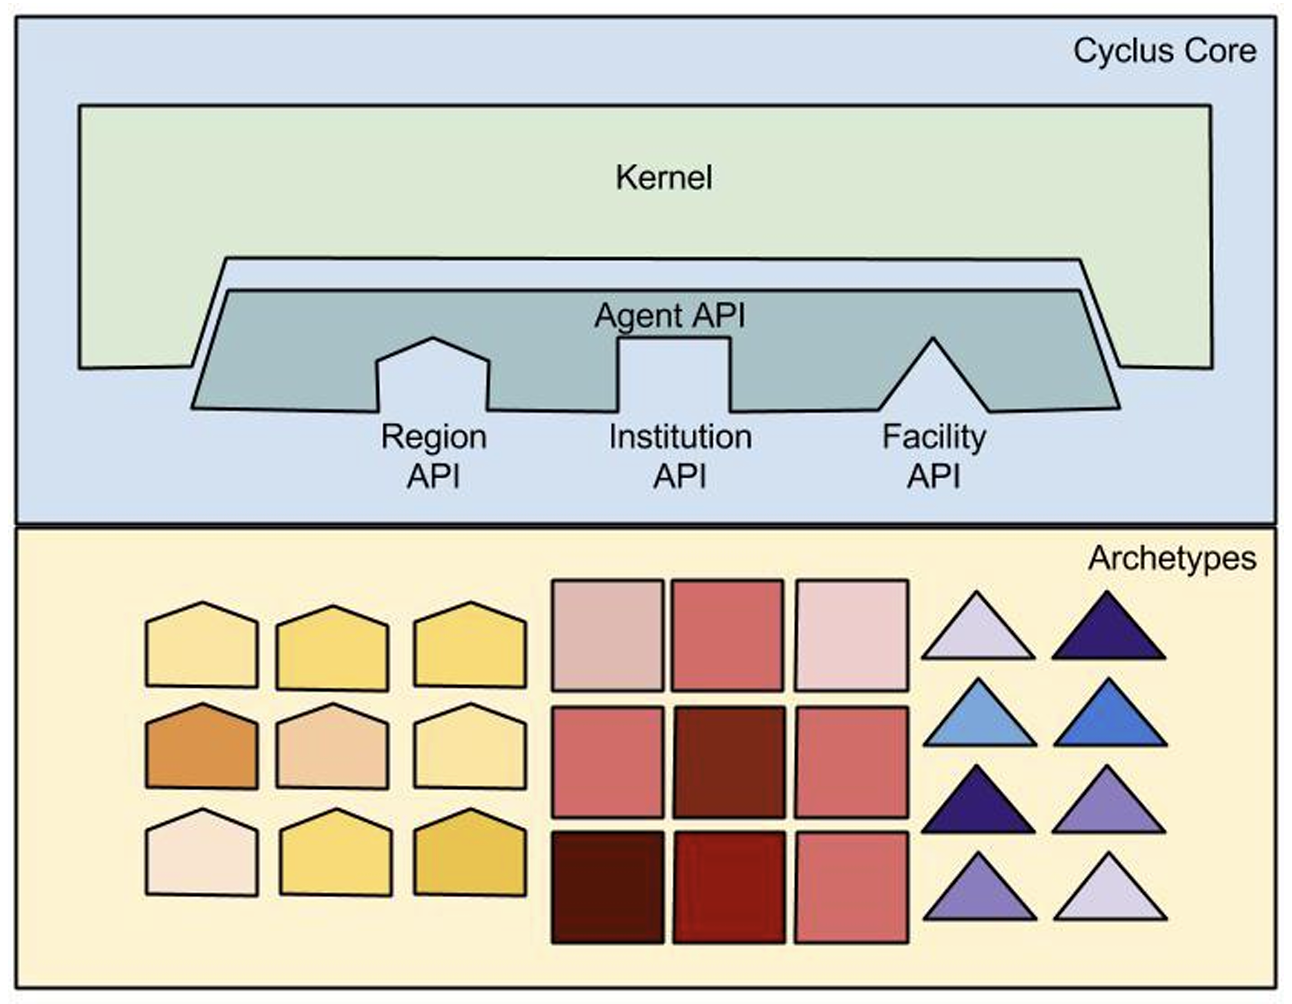
\includegraphics[width=1.0\textwidth]{figures/Cyclus.png}
        \end{center}
        \caption{The Cyclus core offers APIs that simplify kernel interactions, allowing archetypes to be loaded modularity into the simulation.~\cite{huff_fundamental_2016}}
        \label{fig8}
    \end{figure}

    A central objective of this work is to quantify the fuel-cycle performance of XDS technologies at isotopic resolution. 
    Achieving this requires realistic input streams that reflect the current and projected isotopic compositions, burnup histories, 
    and decay corrected radionuclide inventories of spent fuel discharged from commercial reactors. Using the updated 
    STANDARDS 5.0.1 dataset (formerly UNF-ST\&DARDS), age corrected isotopic vectors are used to construct representative SNF 
    compositions that capture the effects of burnup, initial enrichment, fuel type, and decay time. 
    These data form the basis for establishing XDS input streams and for disaggregating the national SNF inventory into resource 
    classes that vary in transuranic content, radiotoxicity, or suitability for transmutation. In this way, 
    Cyclus simulations can distinguish which portions of the national inventory hold the highest potential value for Minor Actinides (MA) burning 
    XDS concepts.\\

    To support these objectives, a dedicated U.S. inventory module is being developed within Cyclus. This module is designed to 
    represent the national waste inventory as a dynamic storage type facility that holds SNF categorized and parameterized 
    according to the latest STANDARDS dataset. Within the module, each fuel batch is stored as a material object with an 
    associated mass, isotopic composition, and decay history. The module enables external Cyclus facilities, such as 
    ADS reactors to request material based on user defined specifications. When material is supplied, the inventory is 
    automatically updated to reflect removal of the requested mass and isotopics. This functionality allows scenario 
    studies to explore how much of the national inventory could be processed, the rate at which materials are consumed, 
    and how inventory composition evolves over time as different technologies are deployed.\\

    Parallel to the inventory module, an XDS facility module is under development to represent accelerator driven systems 
    capable of consuming transuranic rich SNF. This module is structured to accommodate a range of ADS design concepts, 
    including different target materials, coolant types, and fuel compositions. The first implementation is based on the 
    ADS configuration proposed at Argonne National Laboratory. Within Cyclus, the ADS module receives material from the 
    U.S. inventory module, processes it according to user specified operating parameters, and tracks the resulting mass reduction, 
    changes in isotopic composition, and key performance metrics such as minor actinide destruction rate, energy production, 
    and waste radiotoxicity reduction. The combination of these two modules one representing the national inventory and 
    the other representing consumption pathways enables system level evaluation of how ADS deployment scales, how many 
    units are needed to achieve specific waste reduction goals, and how quickly the inventory could be transmuted under 
    different scenarios.\\

\begin{figure}[H]
\centering
\resizebox{0.95\textwidth}{!}{%
\begin{tikzpicture}[
    >=Stealth,
    node distance=3.2cm,
    block/.style={
        draw,
        rounded corners,
        minimum width=3.4cm,
        minimum height=1.4cm,
        align=center
    },
    annot/.style={font=\footnotesize, align=center}
]

%-------------------- NODES (top row) --------------------%
\node[block] (inv) {Inventory\\STANDARDS 5.0.1};
\node[block, right=of inv] (sep) {Separation\\Facility};
\node[block, right=of sep] (mix) {Mixer\\Facility};
\node[block, right=of mix] (xds) {XDS\\Facilities};

% bottom row
\node[block, below=3.0cm of mix] (stor) {Storage\\Facility};
\node[block, below=2.0cm of stor] (reproc) {Reprocessing\\Facility};

%-------------------- ARROWS --------------------%

% Inventory -> Separation Facility
\draw[->] (inv) -- (sep)
    node[midway, above, annot]{Assemblies}
    node[midway, below, annot]{\& composition};

% Sep Facility -> Mixer (MA, LLFPs, else)
\draw[->] (sep.east) ++(0,0.5) -- ([yshift=0.5cm]mix.west)
    node[midway, above, annot]{MAs};
\draw[->] (sep.east) -- (mix.west)
    node[midway, above, annot]{LLFPs};
\draw[->] (sep.east) ++(0,-0.5) -- ([yshift=-0.5cm]mix.west)
    node[midway, above, annot]{else};

% Mixer -> XDS
\draw[->] (mix) -- node[above, annot]{Based on design} (xds);

% XDS -> Storage
\draw[->] (xds.south) |- (stor.east);

% XDS -> Reprocessing
\draw[->] (xds.south) |- (reproc.east);

% Separation -> Storage (unwanted composition), define junction
\draw[->] (sep.south)
  -- ++(0,-3.7) coordinate (sepstor)
  -- (stor.west)
  node[pos=0.7, left, annot]{unwanted\\composition};

% Reprocessing -> junction on line to Storage
\draw[->, dashed] (reproc.west) -| (sepstor);

\end{tikzpicture}%
}
\caption{Conceptual flow from UNF-STANDARDS inventory to XDS, storage, and reprocessing.}
\end{figure}

    Together, these modules create a quantitative framework linking the detailed SNF characterization performed in this report 
    with forward looking fuel cycle analyses. By embedding accurate isotopic compositions derived from STANDARDS data into 
    Cyclus simulations, it becomes possible to evaluate XDS system designs, assess trade offs among accelerator or target 
    configurations, compare transmutation strategies, and measure their aggregate impact on the U.S. waste inventory. 
    This integration ensures that future scenario analyses are grounded in realistic, data driven representations of 
    the commercial and DOE-managed SNF resources, enabling robust evaluation of advanced fuel cycle strategies.\\

    The isotopic feed streams used for XDS transmutation in Cyclus are derived directly from the STANDARDS 5.0.1 dataset at representative discharge burnups 
    (40–60 GWd/MTU for PWR fuel and 30–50 GWd/MTU for BWR fuel), with decay corrections applied to match the assumed spent fuel cooling time. 
    For scenarios focused strictly on minor actinide (MA) reduction, the feed consists of the isotopes that dominate long term radiotoxicity, decay heat, 
    and neutron absorption in the commercial SNF inventory: uranium (U-235, U-238), plutonium (Pu-238 through Pu-242), neptunium-237, 
    americium (Am-241, Am-242m, Am-243), and curium (Cm-244 through Cm-247). Plutonium isotopes are included to maintain the subcritical multiplication 
    factor of the XDS, while the MA vector represents the primary target for transmutation. In some XDSs designs, technetium-99 and iodine-129 are 
    also incorporated in the feed because of their strong spectral-shaping effects.~\cite{gohar_ads_2021}\\

    A second, extended feed stream is used for XDS concepts that aim to simultaneously transmute long lived fission products (LLFPs) alongside actinides. 
    In this scenario the MA composition described above is supplemented with selected LLFP isotopes that significantly influence long term radiotoxicity or 
    neutron economy, including Tc-99, I-129, Cs-135, Se-79, Sn-126, Zr-93, Pd-107, Kr-85, and Sm-151. 
    These LLFPs are incorporated only when the system design explicitly targets LLFP destruction; 
    otherwise they appear solely as fission products generated during irradiation. 
    Together, the MA-only and MA+LLFP feed definitions allow Cyclus to represent a spectrum of XDS concepts ranging from conservative 
    actinide burner designs to more aggressive, waste reduction strategies. For molten-salt-based XDS systems, 
    the precise feed composition also reflects chemical compatibility requirements, 
    including the redox potential and solubility of dissolved actinides or surrogate fluorides in the carrier salt.~\cite{herrera-martinez_transmutation_2007}\\

    The output stream generated by the XDS facility in Cyclus represents the “spent fuel” of the ADS irradiation stage and captures the isotopic changes 
    that occur during transmutation. Following irradiation, the material contains reduced quantities of minor actinides, particularly Am-241, Am-243, Np-237, 
    and multiple curium isotopes, which reflects the primary transmutation objective of the system. 
    The plutonium vector evolves through a combination of fission and neutron capture reactions, typically showing reduced Pu-239 and Pu-241 and corresponding growth in Pu-240 and Pu-242. 
    When LLFP transmutation is not activated in the scenario, long lived isotopes such as Tc-99, I-129, Sn-126, and Pd-107 remain in the output inventory. 
    Overall, the resulting composition demonstrates substantial actinide mass reduction, increased fission product content, and a modified transuranic vector, 
    providing a physically realistic representation of XDS discharge material for further processing, storage, or reinsertion into subsequent fuel cycle stages.~\cite{noauthor_proceedings_nodate}


%%%%%%%%%%%%%%%%%%%%%%%%%%%%%%%%%%%%%%%%%%%%%%%%%%%%%%%%%%%%%%%%%%%%%%%%%%%%%%%%%%%%%%%%%%%%%%%%%%%%%%%%%%%%%%%%%%%%%%%%%%%%%%%%%%%%%%%%%%%%%%%%%%%%%%%%%%%%%%%%%%%%%
%%%%%%%%%%%%%%%%%%%%%%%%%%%%%%%%%%%%%%%%%%%%%%%%%%%%%%%%%%%%%%%%%%%%%%%%%%%%%%%%%%%%%%%%%%%%%%%%%